\documentclass[presentation]{beamer}
%\documentclass[presentation]{beamer}

\usecolortheme{Imperial}
 
\usepackage[utf8]{inputenc}
\usepackage[english]{babel}

\DeclareGraphicsExtensions{{.eps}}
\graphicspath{{./fig/}}

\usepackage[style=authoryear]{biblatex}
\renewcommand*{\bibfont}{\footnotesize}

\newcommand{\bs}{\mathbf} %\mathbf \boldsymbol
\newcommand{\NN}{{\mathcal{N}}}
\def\bphi{\boldsymbol{\phi}}
\def\bpsi{\boldsymbol{\psi}}
\def\bmu{\boldsymbol{\mu}}
\def\bsigma{\boldsymbol{\sigma}}
\def\bdelta{\boldsymbol{\delta}}
\def\bgamma{\boldsymbol{\gamma}}
\def\bxi{\boldsymbol{\xi}}
\def\blambda{\boldsymbol{\lambda}}
\def\btau{\boldsymbol{\tau}}
\def\bomega{\boldsymbol{\omega}}
\def\brho{\boldsymbol{\rho}}
\newcommand{\commentout}[1]{}

\newcommand{\mean}[1]{\mathbf{E}\left[#1\right]}
\newcommand{\inv}[1]{{#1}^{-1}}
\DeclareMathOperator{\rank}{\mathrm{rank}}
\DeclareMathOperator{\cov}{\mathrm{Cov}}
\DeclareMathOperator{\var}{\mathrm{Var}}
%\DeclareMathOperator{\col}{\mathrm{col}}
\newcommand{\col}[1]{\underset{{#1}}{\mathrm{col}}}
\newcommand{\row}[1]{\underset{{#1}}{\mathrm{row}}}
\newcommand{\diag}[1]{\underset{{#1}}{\textrm{diag}}}

%%%%% Define symbols for estimates - we may want to change them, and this could make it easier
\newcommand{\est}[2]{\tilde{#1}_{[#2]}}
\newcommand{\err}[1]{\epsilon_{[#1]}}
\newcommand{\res}[1]{r_{[#1]}}
\newcommand{\thr}[2]{\bar{#1}_{[#2]}}

% complying UK date format, i.e. 1 January 2001
\usepackage{datetime}
\let\dateUKenglish\relax
\newdateformat{dateUKenglish}{\THEDAY~\monthname[\THEMONTH] \THEYEAR}

% -----------------------------------------------------------------------------

\title{A Distributed Approach for the Detection of Covert Attacks in Interconnected Systems with Stochastic Uncertainties}
%\subtitle{Subtitle}
\author{\textbf{Angelo Barboni}, Alexander J. Gallo, Francesca Boem, Thomas Parisini}
\date{27 June 2019}

\addbibresource{extra.bib}
\addbibresource{CDC19.bib}

\begin{document}
 
\begin{frame}[noframenumbering,plain]
\titlepage
\end{frame}

\begin{frame}[noframenumbering,plain]{Outline}
    \tableofcontents
\end{frame}

\section{Introducing the Problem}

\begin{frame}{Introduction}
\begin{itemize}
    \item<1-> Security is a crucial problem for safe and reliable operation of critical infrastructure.
    \item<2-> Problem formulated in \parencite{mo2010false,teixeira2015secure,Pasqualetti2015}.
    \item<3-> See \parencite{dibaji2019systems} for a recent review.
    \item<4> Centralized architectures have received significant attention, distributed ones not as much. 
\end{itemize}
\end{frame}

\subsection{Large-Scale Systems}

\begin{frame}{Interconnected Large-scale Systems}
\begin{itemize}
    \item $N$ subsystems $\mathcal S_i$ equipped with controllers $\mathcal C_i$ and diagnosers $\mathcal D_i$.
    \item Communication pattern mirrors physical interconnection.
    \item Local neighborhood $\mathcal N_i$.
\end{itemize}
\begin{center}
    \includegraphics[scale=1]{fig/cdc19arch.pdf}
\end{center}
(e.g. $N=4$, $\mathcal N_1 = \{4\}$, $\mathcal N_2 = \{3,4\}$, etc.)
\end{frame}

%\begin{frame}{}
%\begin{block}{}
%\centering
%Malicious activity aimed at disrupting operation, counterfeiting data, or acquiring confidential information of a system.
%\end{block}
%\bigskip

%\textbf{Focus}: signal injections on control and measurement channels

%\bigskip
%\centering
%\includegraphics[scale=0.5]{twodist-attack-uy.eps}
%\end{frame}

\begin{frame}{Local Model}

\begin{equation*}
    \mathcal S_i:\left\lbrace
    \begin{aligned}
    	x_i(k+1) &= A_ix_i(k) + B_i \textcolor{red}{\tilde u_i(k)} + \sum_{j \in \mathcal N_i}A_{ij}x_j(k) + w_i(k)\\
        y_i(k) &= C_ix_i(k) + v_i(k)
    \end{aligned}\right.
\end{equation*}

\begin{minipage}[c]{0.51\linewidth}
Attacker $\mathcal A_i$ injects $\eta_i, \gamma_i$:
\begin{equation*}
    \begin{aligned}
    	\textcolor{red}{\tilde y_i} &\doteq y_i - \textcolor{red}{\gamma_i}  \\
        \textcolor{red}{\tilde u_i} &\doteq u_i + \textcolor{red}{\eta_i}
    \end{aligned}
\end{equation*}
\begin{itemize}
    \item $\mathcal S_i$ driven by $\textcolor{red}{\tilde u_i}$, outputs $y_i$
    \item $\mathcal D_i$ and $\mathcal C_i$ use $\{\textcolor{red}{\tilde y_i}, u_i\}$
\end{itemize}
\end{minipage}%
\begin{minipage}[c]{0.48\linewidth}
    \centering
    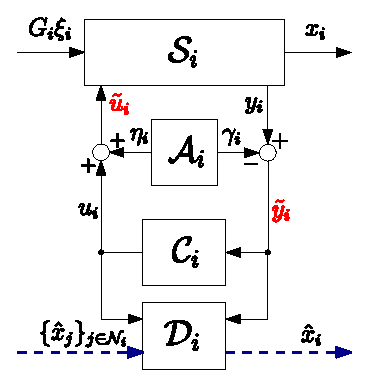
\includegraphics[scale=.7]{fig/cdc19-subsys.eps}
\end{minipage}
\end{frame}

\begin{frame}{Local Model}
\begin{itemize}
    \setlength{\itemsep}{2ex}
    \item<1-> $w_i \sim \mathcal{N}(0,W_i)$ and $v_i \sim \mathcal{N}(0,V_i)$ are i.i.d. Gaussian, $x_i(0)\sim \mathcal{N}(\bar{x}_i^0,\Pi_i^0)$, with $\Pi_i^0 > 0$ and $\bar{x}_i^0$ known and independent from $w_i$ and $v_i$.
    \item<2->$C_i$ are such that $\rank(C_iG_i) = \rank(G_i) = g_i$, where
        $$
        \sum_{j\in\mathcal{N}_i}A_{ij} x_j = \row{j\in\NN_i}\left[A_{ij}\right]\col{j\in\NN_i}\left[x_j\right] = G_i \bar{E}_i \zeta_i = G_i \xi_i
        $$
    i.e. we project \emph{only the independent components} of the interconnections.
    \item<3> Partition a signal into \emph{healthy} and \emph{attacked} components, e.g. $y_i = y_i^h + y_i^a$.
\end{itemize}

\end{frame}

\subsection{Covert Attacks}

\begin{frame}{Covert Attacks}    
Introduced by \parencite{smith2011decoupled} for the centralized case in the frequency domain.
\vfill
\begin{block}{Definition}
The agent $\mathcal A_i$ is covert if the attacked (viz. $\eta_i$, $\gamma_i \neq 0$) measurement output $\tilde y_i$ cannot be distinguished from the nominal system response:
$$  \tilde{y}_i(k) = y_i^h(k) = C_ix_i^h(k) + v_i(k) $$
\end{block}
\vspace{3ex}
Possible strategy: \emph{superimpose $\eta_i$ and compensate with $\gamma_i$}.

\end{frame}

\begin{frame}{Internal Adversary Model}
We model $\mathcal A_i$ as a dynamical system:
\begin{equation*}
    \tilde{\mathcal{S}}_i : \left\lbrace
    \begin{aligned}
    	&x^{a}_i(k+1) = A^a_i x^a_i(k) + B^a_i \eta_i(k) \\
        &\gamma_i(k) = C^a_i x^a_i(k) \,
    \end{aligned}\right. 
\end{equation*}
with $\eta_i$ the \emph{unknown} (to the defender) control input.
\bigskip
\begin{block}{Assumption 1}
The attacker has \emph{perfect knowledge} of $\mathcal S_i$: $(A^a_i, B^a_i, C^a_i) = (A_i,B_i,C_i)$.
\end{block}
\begin{block}{}
Let $k_a$ be the time of attack, Assumption 2 and $x^a_i(k_a) = 0$ are sufficient for $\mathcal A_i$ to be covert.
\end{block}
\end{frame}


\begin{frame}[c]{Example}
\centering
\vspace{2ex}
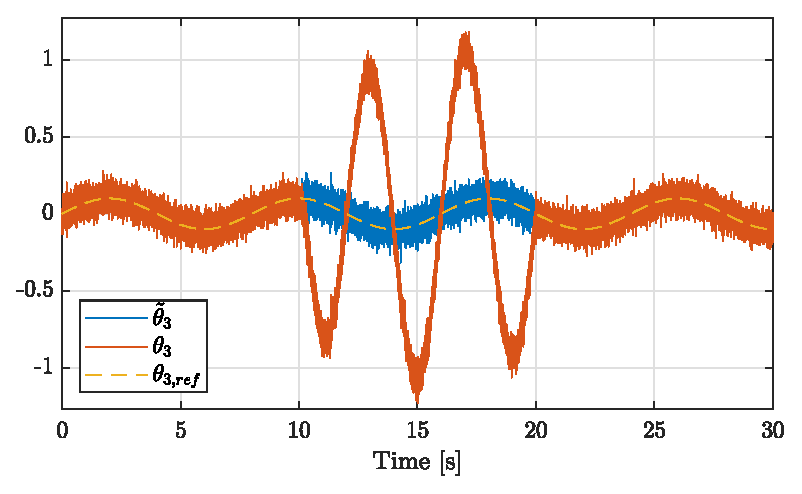
\includegraphics[height=0.65\paperheight]{fig/trajectories-pres.eps}    
\end{frame}

\subsection{Problem Statement}

\begin{frame}{Problem Statement}
\begin{block}{Problem}
    \centering\large
    Covert attacks are undetectable by \emph{any local} monitoring system.
\end{block}

\vspace{4ex}
\begin{alertblock}{Objective}
    \centering\large
    Design a  
    \textbf{distributed, model-based}  detection scheme 
    to detect attacks that are \emph{locally} covert.
\end{alertblock}
\end{frame}

\AtBeginSection[]
{
  \begin{frame}[noframenumbering,plain]{Outline}
    \tableofcontents[currentsection]
  \end{frame}
}

\section{Proposed Solution}

\subsection{Exploiting Physical Connections}

\begin{frame}{Basic Idea}
\centering
\vspace{1.5ex}
\includegraphics[height=0.5\paperheight]{fig/cdc-concept.pdf}
\vspace{1.5ex}
\begin{block}{}
\begin{enumerate}
    \item Obtain an estimate $\hat\xi_i(k-1)$ of neighboring ``states'' $x_j(k-1)$ that explains the current local state $x_i(k)$
    \item Compare such an estimate with \emph{communicated} estimates $\hat x_j$
\end{enumerate}
\end{block}
\end{frame}

\subsection{Detector Design}

\begin{frame}{Step 1: Joint Input and State Estimator}
Solve an Unbiased Minimum Variance Estimation problem (see~\cite{kitanidis1987unbiased,gillijns2007unbiased}).

\bigskip
Obtain the filter:
\begin{align*}
        &\hat{x}_i(k) =  \bar{A}_i(k)\left[A_i\hat{x}_i(k-1) + B_i u_i(k-1)\right] + \bar L_i(k) \tilde y_i(k) \\
	    &\hat{\xi}_i(k-1|k) = M_i(k)\left[\tilde{y}_i(k) - C_i \left(A_i\hat{x}_i(k-1) + B_i u_i(k-1)\right) \right],
\end{align*}
with 
$$
     \bar{L}_i(k) \doteq K_i(k) + \left(\mathbf{I} - K_i(k) C_i \right)G_iM_i(k)
$$ 
and
$$
     \bar{A}_i(k) \doteq \mathbf{I} - \bar{L}_i(k)C_i.
$$
\end{frame}

\begin{frame}{Existence Conditions}
\begin{block}{Lemma 1 (\cite[Thm.12]{gillijns2007unbiased})}
If $M_i(k)$  satisfies
$$M_i(k)C_iG_i = \mathbf{I}_{g_i} \, , \quad \forall k \geq 0.$$
then $\hat{\xi}_i$ and $\hat{x}_i$ are unbiased estimates of $\xi_i$ and $x_i$, minimizing the mean square error over the class of all linear unbiased estimates based on $\bar{x}_i^0$ and $y_i(\kappa), 0\leq \kappa\leq k$.
\end{block}
\vspace{4ex}
\begin{block}{}
The rank decomposition $G_i\bar E_i$ guarantees that the lemma holds, on the other hand \emph{only} $\rank(E_i)$ components can be estimated. 
\end{block}
\end{frame}

\begin{frame}{State Estimation Error Analysis}
\onslide<1->{
The error $\epsilon_i(k) \doteq x_i(k) - \hat{x}_i(k)$ is such that
\begin{itemize}
    \item \textbf{No attack}: $\mean{\epsilon_i(k)} = 0, \var(\epsilon_i(k)) = \Pi_i(k)$
    \item \textbf{Under attack}: $\mean{\epsilon_i(k)} = x_i^a(k), \var(\epsilon_i(k)) = \Pi_i(k)$ (attack is deterministic)
\end{itemize}}

\vspace{2ex}
\onslide<2->{
Note that
\begin{itemize}
    \item $\epsilon_i(k)$ (and the corresponding residual $r_i(k) = C_i\epsilon_i(k)$) are not accessible!
    \item The \emph{available} residuals $\tilde r_i(k) = \textcolor{red}{\tilde y_i(k)} - C_i\hat{x}_i(k)$ are the same with and without attack. 
\end{itemize}}

\vspace{2ex}
\begin{block}{}<3->
A local state observer is not capable alone of detecting a covert attack.
\end{block}
\end{frame}

\begin{frame}{Coupling Estimation Error Analysis}
\onslide<1->{
For $\rho_i(k-1|k) \doteq \xi_i(k-1) - \hat\xi_i(k-1|k)$
\begin{itemize}
    \item \textbf{No attack on $\mathcal S_j$}: $\mean{\rho_i(k-1|k)} = 0, \var(\rho_i(k-1|k)) = \Delta_i(k)$
    \item \textbf{$\mathcal S_j$ Under attack}: $\textcolor{red}{\mean{\rho_i(k-1|k)} \propto x_j^a(k)}, \var(\rho_i(k-1|k)) = \Delta_i(k)$ 
\end{itemize}}

\vspace{3ex}
\begin{block}{Distributed residual}<2->
$\rho_i$ is not available! We need to enable communication to obtain an estimate
$$ \hat \rho_i(k-1|k) \doteq  \hat \xi_i(k-1|k) - \bar{E}_i \col{j\in\NN_i}[\hat x_j(k-1)] $$
\end{block}
\end{frame}

\subsection{Detection Strategy}

\begin{frame}{Properties of $\hat\rho_i$}
    \begin{block}{Proposition}
        Let Lemma 1 hold and suppose a subsystem $\mathcal S_l, l \in \mathcal N_i$ is attacked at time $k_a$.
        The residual $\hat \rho_i(k-1|k)$ follows a Gaussian distribution with mean and variance $\mu_i(k)$ and $\Sigma_i(k) > 0$, respectively, where 
\begin{align*}
    &\mu_i(k) = \left\lbrace
        \begin{aligned}
            &0, &&k \leq k_a, \\
            &\zeta_{i,l}^a(k-1) &&k > k_a.
        \end{aligned}\right.\\[2ex]
    &\Sigma_i(k) =  \bar{E}_i\diag{j\in\NN_i}\left[\Pi_j(k-1)\right]\bar{E}_i^\top + \Delta_i(k-1|k) \quad \forall k, 
\end{align*}
where $\zeta_{i,l}^a(k-1) \doteq \bar E_{i,[l]}x_l^a(k-1)$.  
($\bar E_{i,[l]}$ is the $l$-th row block of $\bar E_i$)
\end{block}
\end{frame}

\begin{frame}{Detection Strategy}
\begin{block}{Assumption 2}
Data exchange between diagnosers is ideal and cannot be attacked.
\end{block}
\vfill
\begin{enumerate}
    \item Consider a detection signal $a_i = \{\mathcal H_i^0, \mathcal H_i^1\}$.
    \item In normal conditions, $a_i$ corresponds to the null hypothesis.
    \item If Subsystem $\mathcal S_j, j \in \mathcal N_i$ is attacked and a \emph{suitable test} passes, then $a_i = \mathcal H_i^1 $.
    \item $a_i$ is broadcast to the neighbourhood $\mathcal N_i$.
    \item If $a_k = \mathcal H_k^1,\, \forall k \in \mathcal N_j$, then $\mathcal S_j$ decides to be under attack.
\end{enumerate}
\end{frame}

\begin{frame}{Suitable Test}
\begin{block}{Local Detection Problem}<1->
    The detection logic in $\mathcal{D}_i$ accepts one of the following hypotheses:
    \begin{equation*}
        \begin{aligned}
            &\mathcal{H}_i^0: \hat \rho_i(k-1|k) = \hat\rho_i^h(k-1|k), \\
            &\mathcal{H}_i^1: \hat \rho_i(k-1|k) = \hat\rho_i^h(k-1|k) + \zeta_{i,l}^a(k-1).
        \end{aligned}
    \end{equation*}
\end{block}

\bigskip
\onslide<2->
The problem is equivalent to detecting an unknown signal embedded in white Gaussian noise.
Set up a GLRT over a window of $\omega_i$ samples: hypothesis $\mathcal H_i^1$ is accepted when 
\small{
    $$ T(\hat\rho_i,k) \doteq \log \frac{p\left(\hat \rho_i(k-1|k) \left| \hat \zeta_{i,l}^a(k-\omega_i), \dots, \hat \zeta_{i,l}^a(k-1), \mathcal H_i^1\right)\right.}{p\left(\hat \rho(k-1|k) \left| \mathcal H_i^0\right)\right.} > \theta_i(k) $$
}
\onslide<3>
\emph{Since $\zeta_{i,l}^a$ is white}, $\hat \rho_i(k-1|k) = \hat\zeta_{i,l}^a(k-1)$ is a ML estimate.
\end{frame}

\begin{frame}{Test Implementation}
\onslide<1->
Since $\Sigma_i > 0$, there exists an orthogonal diagonalization $\Sigma_i(k) = U_i(k) \Lambda_i(k) U_i^\top(k)$. 

\smallskip
Define ${\hat z_i(k) \doteq U_i(k) \hat\rho_i(k)} \Rightarrow T^\prime(\hat z_{i[q]},k) > \bar\theta_{i[q]}(k).$
\onslide<2->
\bigskip
By construction, $T^\prime$ is $\chi^2$ distributed with degrees of freedom $\omega_i$ and non-centrality parameter $\nu_q$ :
\begin{equation*}
    T^\prime(\hat z_{i[q]},k) \sim \left\lbrace
    \begin{aligned}
        &\chi^2_{\omega_i}(0) \qquad&&\text{if }\mathcal H^0,\\
        &\chi^2_{\omega_i}(\nu_q) &&\text{if }\mathcal H^1,
    \end{aligned}\right.
\end{equation*}
\begin{block}{}<3->
Thresholds $\bar\theta_{i[q]}(k)$ can be computed for a given probability of false alarm.
\end{block}
\begin{block}{}<4->
$\nu_q$ depends on the energy of the attacked state $x_l^a$, scaled by the corresponding interconnection weight. As $\nu_q \rightarrow 0$, the probability of detection approaches that of false alarm.
\end{block}
\end{frame}

%\begin{frame}{Threshold Selection and Remarks}
%\begin{itemize}
%    \setlength{\itemsep}{2ex}
%    \item<1-> Since the distribution of $T^\prime(\hat z_{i[q]},k)$ is known, we can find a threshold $\bar\theta_{i[q]}$ by assigning a desired probability of false alarm:
%    $$ 
%    \mathrm{P}_{i[q]}^f(k) =  \Phi\left(\frac{1}{\sqrt{2\omega_i}}\left( \frac{\bar\theta_{i[q]}}{\lambda_{i[q]}} - \omega_i\right) \right)
%    $$
%    \item<2-> Overall probability of false alarm can be found as well.
%    \item<3>
%\end{itemize}
%\end{frame}

\begin{frame}[c]{Caveat}
\begin{itemize}
    \setlength{\itemsep}{2ex}    
    \item<1-> Multiple covert attacks in the same neighborhood may not be detected if the attackers compensate each other (this violates locality of Assumption 1).
    
    \item<2> Additional condition on connectivity for isolation: $\mathcal N_i \not\subseteq \mathcal N_j,\, \forall i \neq j \in \{1 ,\dots, N \} $\\[2ex]
    \begin{minipage}{0.48\linewidth}
        \centering
        \scalebox{1}{
            \begin{tikzpicture}
                \tikzstyle{every node}=[draw,shape=circle,scale=0.8,fill=white]
                \def\tip{{Latex[scale=1]}}
                
                \node (n1) at (0, 1) {\textcolor{red}{1}};
                \node (n2) at (1, 0)  {2};
                \node (n3) at (0, -1)  {\textcolor{darkgreen}{3}};
                \node (n4) at (-1 , 0)  {4};
                \foreach \from/\to in {n2/n1,n3/n2,n4/n3,n1/n4}
                \draw[\tip-\tip] (\from) -- (\to);
            \end{tikzpicture}
            }
        \end{minipage}
        \begin{minipage}{0.48\linewidth}
            $\mathcal N_2 = \mathcal N_4 = \{1,3\} \Rightarrow$ \\
            $\mathcal S_1 \text{ or } \mathcal S_3$ attacked
        \end{minipage}
    
\end{itemize}
\end{frame}

\section{Example and Concluding Remarks}
 
\begin{frame}{Example -- Spring-connected pendula}
	\begin{equation*}
		m_il_i^2\Ddot{\delta}_i = m_igl_i\delta_i + u_i + \sum_{j\in\NN_i} k_{ij}a_i^2(\delta_j-\delta_i)
	\end{equation*}
	
	Discretize each subsystem using Euler's approximation with sampling time $T_s = 0.01$ s. %Variance matrices $W_i = 10^{-3}\mathbf{I}$ and $V_i = 10^{-3}\mathbf{I}$. 
	
	\vfill
	\begin{columns}
		\begin{column}{0.75\linewidth}
			Attack $\mathcal S_3 $ at $T_a = 35$ s
			$$\eta_3(k) \doteq 0.5 \left(1-e^{-0.3 (k\cdot T_s-k_a)}\right)\,\mathrm{sin}\left(\frac{2}{30} \pi k \cdot T_s\right)$$

			Compensation $\gamma_3$ obtained with exact subsystem model.
		\end{column}
		\begin{column}{0.23\linewidth}
			%\raggedleft
			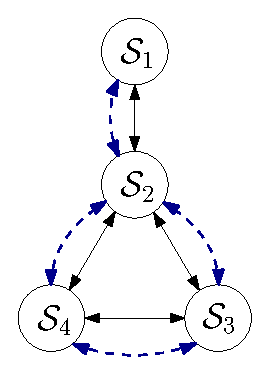
\includegraphics[scale=0.6]{fig/layout.eps}
		\end{column}
	\end{columns}
\end{frame}


\begin{frame}{Example -- Attack detection and isolation}
    
	\begin{columns}
		\begin{column}{0.25\linewidth}
			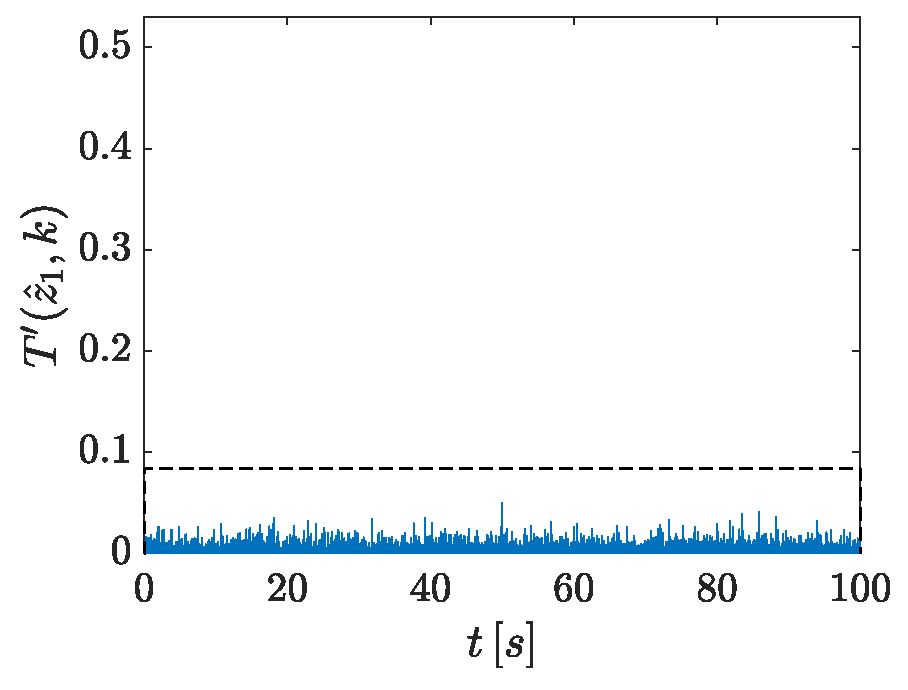
\includegraphics[width=\linewidth]{fig/det1_okThr.eps}
		\end{column}
		\begin{column}{0.25\linewidth}
			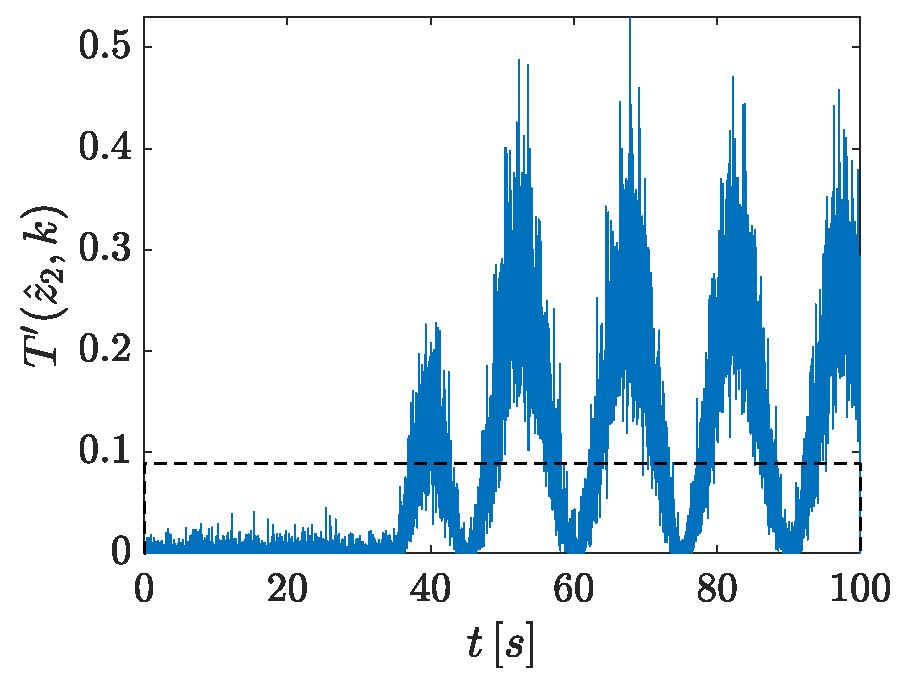
\includegraphics[width=\linewidth]{fig/det2_okThr.eps}
		\end{column}
		\begin{column}{0.25\linewidth}
			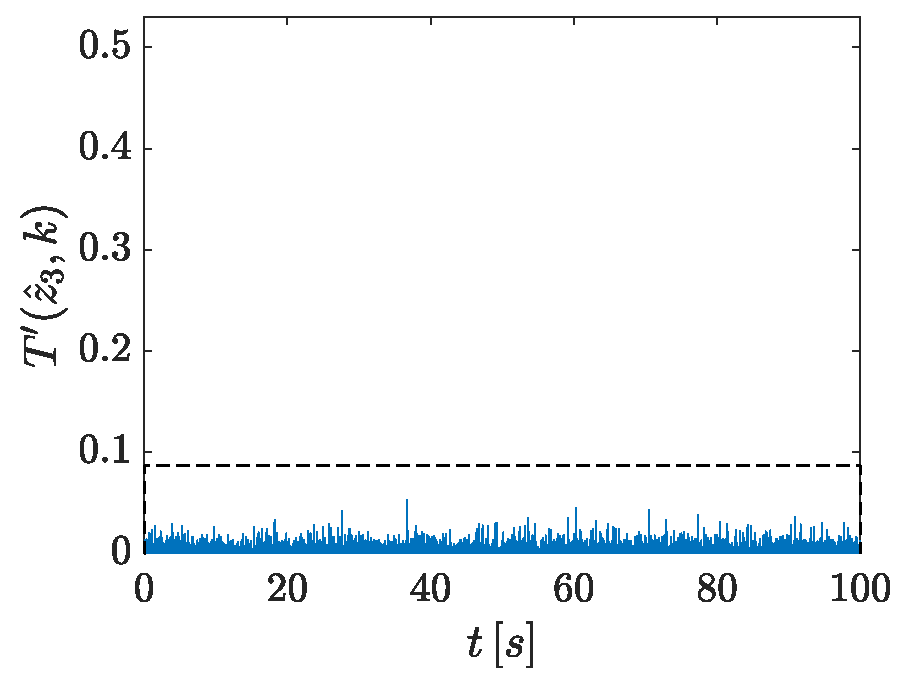
\includegraphics[width=\linewidth]{fig/det3_okThr.eps}
		\end{column}
		\begin{column}{0.25\linewidth}
			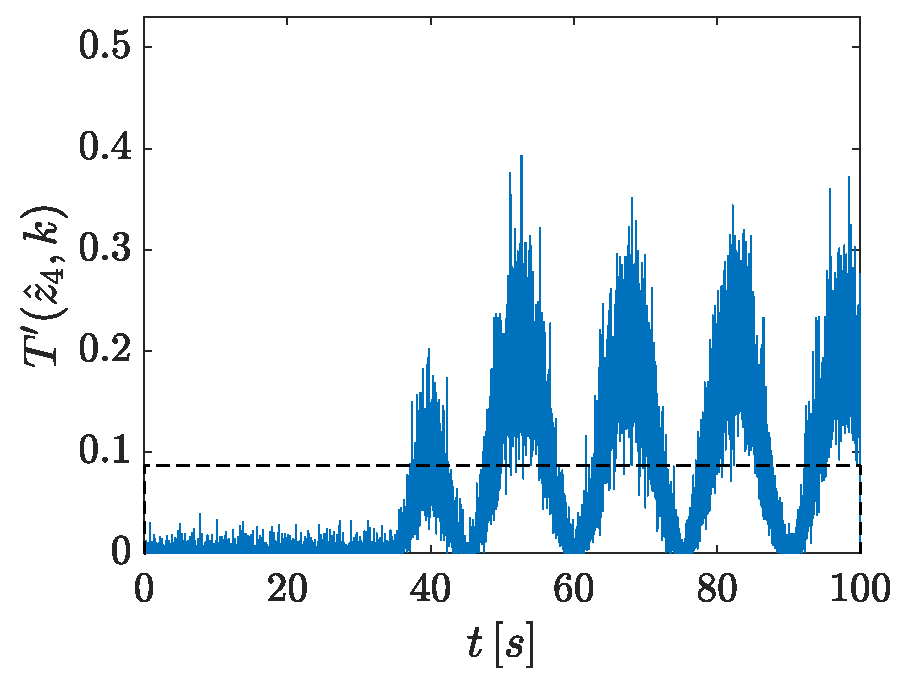
\includegraphics[width=\linewidth]{fig/det4_okThr.eps}
		\end{column}
	\end{columns}
	\begin{center}
	    Comparison of $T^\prime(\hat{z}_i,k)$ with $\bar{\theta}_i(k)$.
	\end{center}
	
	
	\vfill
	Attack is detected by $\mathcal D_2$ at $T_{d,2} = 36.78$~s and by $\mathcal D_4$ at $T_{d,4} = 37.16$~s. 
	At time $T_{isol} = T_{d,4}$, $\mathcal{D}_3$ isolates $\mathcal S_3$ as the attacked subsystem.
	
	\onslide<2>
	\begin{block}{A Note on Isolation}
	    Given the topology of the system, $\mathcal N_1 \subset \mathcal N_3$, and as such $\mathcal D_1$ also isolates $\mathcal{S}_1$ as under attack at time $t = T_{d,2}$.
	   % For time $t \in [T_{d,2},T_{d,4}]$, either $\mathcal S_1$ or $\mathcal{S}_3$ may be under attack, given the detection logic and the architecture of the system.
	\end{block}
\end{frame}

\begin{frame}{Concluding Remarks}
    \begin{itemize}
        \itemsep 2ex
        \item<1-> \textbf{Main point}: physical interconnections and system coupling can be leveraged to reveal attacks that are stealthy on a local scale. %stealthy attacks on a local scale.
        \item<2-> The same principle can be applied to other attacks that comply with the ``covert model'' (i.e. replay attacks)
    \end{itemize}
\end{frame}

\begin{frame}{Future work}
    \begin{itemize}
    \itemsep 1.5ex
        \item Relax the perfect knowledge assumption (robust control framework?)
        \item Relax the ideal communication assumption:
            \begin{itemize}
                \item Unreliable/delay channels.
                \item Attacks on communication (analysis submitted to IFAC2020).
            \end{itemize}
        \item More general models (e.g. switched, nonlinear).
        \item Deeper analysis on connectivity aspects.
    \end{itemize}
\end{frame}

\begin{frame}{Thanks for your attention}
\hbox{\large References:}
\bigskip
\renewcommand*{\bibfont}{\scriptsize}
\printbibliography
\end{frame}

\end{document}

